\section {Simulation Results}

The computer executing the simulation software has the following specifications:

\begin{itemize}
\renewcommand{\labelitemi}{$\bullet$}
\item 2 x Intel Xeon X5550 quad-core Nehalem processors @ 2.66GHz (Hyperthreading enabled)
\item 24GB Memory
\item 2 x Nvidia Tesla T10 boards (half of an S1070)
\item 250GB 7200RPM SATA hard drive

\end{itemize}

As described in the previous section the simulation uses 328 airports in 20 regions. A first
run of the simulation uses 9840 airplanes (30 per airport). Large airports were assigned to
have 6 runways, medium airports were given 3 runways, small airports 2 runways, and non-
bub airports1 runway. Region capacity was also set constant at a maximum of 100 planes per
region. Some statistics from the simulation are shown in table \ref{table:seq_result}.

\begin{table}
\begin{center}
\addtolength{\tabcolsep}{-0pt}
%\tiny
\caption{Sequential Execution Simulation}
\label{table:seq_result}
\begin{tabular}{|c|c|}\hline

Net Events Processed & 2354171  \\\hline
Total Transit Accepted & 14012  \\\hline
Total Transit Rejected & 14288  \\\hline
Total Departure Requests Accepted & 9840 \\\hline
Total Departure Requests Rejected & 1377210 \\\hline
Total Arrival Requests Accepted & 9840 \\\hline
Total Arrival Requests Rejected & 177018 \\\hline

\end{tabular}
\end{center}
\end{table}

Additional experiments were executed increasing the airspace capacity of each region and
the number of runways at each airports. Three additional experiments scale up the capacity
and number of runways by 2, 4, and 8. Figure \ref{fig:seq_req_rejected}, \ref{fig:seq_runtime}, \ref{fig:seq_events} show the number of rejected
departure requests, execution time, and total events processed.



\begin{figure} [htd]
\centering
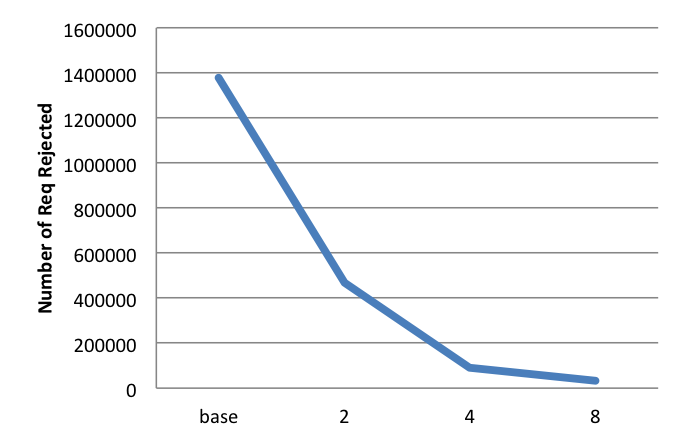
\includegraphics[width=2.5in]{figs/seq_req_rejected.png}
\caption{Number of Rejected Departure Requests}
\label{fig:seq_req_rejected}
\end{figure}

\begin{figure}
\centering
\begin{tabular}{cc}
\begin{minipage}{200pt}
%\frame{\includegraphics[width=200pt]{/Users/chayong/Documents/project2/figs/seq_runtime.png}}
\includegraphics[width=200pt]{figs/seq_runtime.png}
\caption{Sequential Execution Time}
\label{fig:seq_runtime}
\end{minipage}
&
\begin{minipage}{200pt}
%\frame{\includegraphics[width=250pt]{/Users/chayong/Documents/project2/figs/seq_runtime.png}}
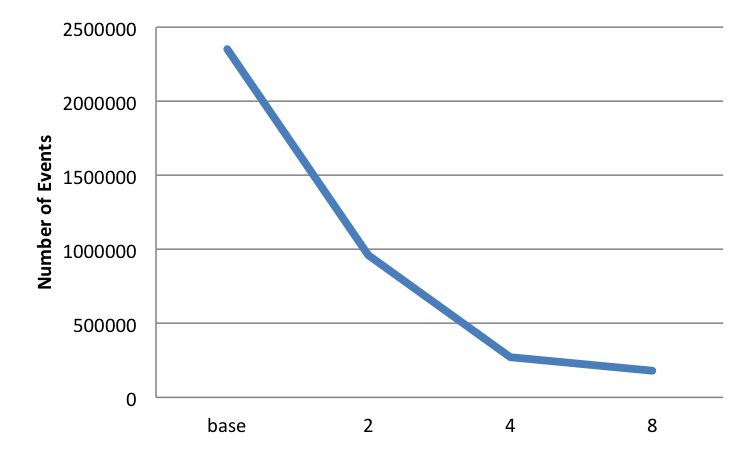
\includegraphics[width=200pt]{figs/seq_events.png}
\caption{Number of Net Events}
\label{fig:seq_events}
\end{minipage}
\end{tabular}
\end{figure}



As expected, by increasing airspace capacity and airport capacity (increasing the number of
runways) the number of rejected departure requests is considerably reduced. Also, execution
time and total events processed also decrease. This can be attributed to the fact that increasing
airspace and airport capacity causes fewer denials for departures, landing, and inter-region
travel.